\chapter{Functions}

\begin{defn}[Function]\label{Function}
A function is the relation between a set of inputs and a set of outputs with the property that each valid input is related to exactly one output. In other words, a function takes  an input value and gives a corresponding output. We denote function $f$ evaluated for a certain $x$ as $f(x)$.
\end{defn}

You have probably seen many functions in previous math classes. Below is a visualization of a function $f$.


%function diagram

\begin{center}
\tikzstyle{decision} = [diamond, draw, fill=blue!20, 
    text width=4.5em, text badly centered, node distance=3cm, inner sep=0pt]
\tikzstyle{block} = [rectangle, draw, fill=blue!20, 
    text width=5em, text centered, rounded corners, minimum height=4em]
\tikzstyle{line} = [draw, -latex']
\tikzstyle{cloud} = [draw, ellipse,fill=red!20, node distance=3cm,
    minimum height=2em]
    
\begin{tikzpicture}[node distance = 2cm, auto]
    % Place nodes
    \node [block] (function) {$f$};
    \node [cloud, left of=function] (input) {$x$};
    \node [cloud, right of=function] (output) {$f(x)$};
    % Draw edges
    \path [line,dashed] (input) -- (function);
    \path [line,dashed] (function) -- (output);
\end{tikzpicture}
\end{center}

In this diagram, $x$ on the left is our input and the $f(x)$ on the right is the output. We can think of $f(x)$ as the function $f$ applied to $x$. Now let's look at a particular function. Let's allow the function $d$ to double any input. Now we have this diagram:

\begin{center}
\tikzstyle{decision} = [diamond, draw, fill=blue!20, 
    text width=4.5em, text badly centered, node distance=3cm, inner sep=0pt]
\tikzstyle{block} = [rectangle, draw, fill=blue!20, 
    text width=5em, text centered, rounded corners, minimum height=4em]
\tikzstyle{line} = [draw, -latex']
\tikzstyle{cloud} = [draw, ellipse,fill=red!20, node distance=3cm,
    minimum height=2em]

\begin{tikzpicture}[node distance = 2cm, auto]
    % Place nodes
    \node [block] (function) {$d$};
    \node [cloud, left of=function] (input) {$1$};
    \node [cloud, right of=function] (output) {$2$};
    % Draw edges
    \path [line,dashed] (input) -- (function);
    \path [line,dashed] (function) -- (output);
\end{tikzpicture}
\end{center}

\noindent
Our new function $d$ takes the input of 1 and gives an output of 2. In other words, the function $d$ doubled our input of 1. When a function acts on a value like this and produces an output, we write $d(1)=2$.

\begin{presentation}
	\begin{defn}[Domain]\label{Domain}
		The domain of a function is the set of all possible inputs that give valid outputs for the function.
	\end{defn}
\end{presentation}

The domain of a function is just a fancy way of saying anything we can put into the function and have the function still work. Consider a paper shredder. If we were to consider this a function, the domain would be paper, credit cards, and late homework. 
\begin{defn}[Range]\label{Range}
	The range of a function is the set of all possible outputs for that function.
\end{defn}

Let's think back to the paper shredder. If the domain of the paper shredder function was paper, credit cards, and late homework, what would be in the range? In other words, what are our possible outputs? In the case of the paper shredder, finding the domain and range are fairly easy since the paper shredder turns all inputs into shredded versions of themselves. However, most of the time this semester, we will be dealing with mathematical functions that have some effect on numerical inputs. The doubling function $d$ is a classic example of this. 

\begin{prblm}[Expressing a function as an equation]\label{Doubling Function}
Using the definition of an equation and your knowledge of the doubling function discussed above, express the function $d$ as an equation. \vspace{4cm}
\end{prblm}

Expressing a function as an equation is going to be the most common way that we look at functions this semester, but not the only way. Sometimes it may be easier to look at and analyze a function using a table of values. 

\begin{presentation}
\begin{example}[Expressing a function using a table of values]\label{Table of Values}
	Think back to the paper shredder function. If wanted to express this function using a table of values, it would like like the following.
\begin{center}
\textbf{Paper Shredder Function} \\
\begin{tabular}{|c|c|c|c|}
\hline
\textbf{input} & paper & credit card & late homework \\
\hline
\textbf{output} & shredded paper & shredded plastic & lower grade \\	
\hline
\end{tabular}
\end{center}

\noindent
 These tables of values become even more useful when dealing with a function that has numerical values. Consider the doubling function $d$.

\begin{center}

\textbf{The Doubling Function} \\
$
\begin{array}{|c|c|c|c|c|c|}
 \hline
 \bm{x} & 1 & 2 & 3 & 4 & 5 \\
 \hline
 \bm{d(x)} & 2 & 4 & 6 & 8 & 10 \\
 \hline
\end{array}
$
\end{center}

\noindent
In some situations, this is the only format in which a function is given to us. Therefore, both reading accurately and creating these tables are important tools for moving forward with functions. 
\end{example}
\end{presentation}

The last major format that functions come in is graphically. 

\pagebreak 

\begin{presentation}
\begin{defn}[Cartesian Plane]\label{The Cartesian Plane}
	The Cartesian Plane is a plane (meaning it's flat) made up of an \color{blue}$x$-axis (the horizontal line) \color{black} and a \color{red} $y$-axis (the vertical line). \color{black}
	\begin{center}
%	\begin{tikzpicture}
%	\begin{axis}[axis background/.style={fill=white}, width=12cm, ymax=10, ymin=-10, xmax=10, xmin=-10, axis lines=middle, grid=major, myaxis, xticklabel style= {font=\tiny, yshift=0.5ex}, yticklabel style={font=\tiny, xshift=0.5ex},xtick={-10,...,10}, ytick={-10,...,10}	]
%	\end{axis}
%	\end{tikzpicture}
	\end{center}
Points on the Cartesian plane are labeled using an $x$-$y$ coordinate. The notation for these coordinates is $(x,y)$. For example, the point with an $x$-value of -4 and a $y$-value of 3 is $(-4,3)$. The point at which the $x$ and $y$ axis meet is called the origin and has an $x$ and $y$ value of 0, giving it the notation $(0,0)$. 

\smallskip
We say that the Cartesian Plane has 4 separate parts, which we call the 4 Quadrants, and are separated by the $x$ and $y$ axes. The first Quadrant is when we have both positive $x$ and $y$ values, which is in the top right corner of the plotted axes above. By moving counterclockwise from the top right, we cross through the second, third, and fourth quadrants in that order. 
\end{defn}
\end{presentation}

\begin{prblm}[Graphing the doubling function]
Let's practice graphing functions by graphing our doubling function $d$, which we already have an equation for (\ref{Doubling Function}).
\vspace{5cm}
\end{prblm}

\begin{presentation}
\begin{example}[Expressing a function using a graph]
Sometimes functions are expressed on the Cartesian Plane. We can use these representation to gather the same information we can get from the others. 
\begin{center}
\begin{tikzpicture}
	\begin{axis}
	%[axis background/.style={fill=white},width=12cm,ymax=10,ymin=-10,xmax=10,xmin=-10,axis lines=middle,grid=major,myaxis,xticklabel style={font=\tiny,yshift=0.5ex},yticklabel style={font=\tiny,xshift=0.5ex},xtick={-10,...,10},ytick={-10,...,10}]
	%	\begin{axis}[axis background/.style={fill=white}, width=12cm, ymax=10, ymin=-10, xmax=10, xmin=-10, axis lines=middle, grid=major, myaxis, xticklabel style= {font=\tiny, yshift=0.5ex}, yticklabel style={font=\tiny, xshift=0.5ex},xtick={-10,...,10}, ytick={-10,...,10}]
	\addplot+[smooth] coordinates {(-2,-8) (-1,-1) (0,0) (1,1) (2,8)};
	%\addplot+[smooth] coordinates {(-2,-8) (-1,-1) (0,0) (1,1) (2,8)};
	\end{axis}
\end{tikzpicture}
\end{center}


This function is the cubic $(x^3)$ function, restricted to the domain -2 to 2. 


\end{example}
\end{presentation}

\begin{presentation}
\begin{defn}[Intercepts]\label{Intercept}
	An intercept of a function is a point where the function crosses (or intercepts) any axes. A function can have multiple intercepts.
\end{defn}
\end{presentation}

When talking about intercepts, we usually distinguish between the $x$-intercepts and the $y$-intercept.

\begin{prblm}
What must be the $y$ coordinate of a $x$-intercept? How do we know this? What must be the $x$ coordinate for the $y$-intercept?	
\vspace{4cm}
\end{prblm}

\newpage
\begin{prblm}

Consider the following function:
\begin{center}
\begin{tikzpicture}
	\begin{axis}
	%[axis background/.style={fill=white}, width=12cm, ymax=10, ymin=-10, xmax=10, xmin=-10, axis lines=middle, smooth, grid, myaxis, xticklabel style= {font=\tiny, yshift=0.5ex}, yticklabel style={font=\tiny, xshift=0.5ex},xtick={-10,...,10}, ytick={-10,...,10}]
	\addplot[color=red] coordinates {(-9,0) (-8, 1) (-4, 6) (-2, 4) (0, 5) ( 2, 3) (4, 0) (5, -2) (8, -6)};	
	\addplot[mark=*, color=red] coordinates {(-9,0)};
	\addplot[mark=*, color=red] coordinates {(8, -6)};
	\end{axis}
\end{tikzpicture}
\end{center}

\noindent
What is the domain of this function? What about the range? What are the intercepts of the function?
\vspace{4cm}
\end{prblm}


\pagebreak


\section*{Exercises}

\begin{exercise}
For the following functions, find $f(3)$:

\begin{itemize}
\item $f(t) = 4t$
\item $f(t) = -\frac{1}{2}t + 1$
\item $f(x) = x^2 - 2x + 1$
\item $f(x) = 2$
\item $f(z) = 7$
\item $f(z) = z^3-z^2-z-1$
\end{itemize}

\end{exercise}
\bigskip

\begin{exercise}
Build a table for the following functions:

\begin{itemize}
\item $f(t) = t + t + t + t + t$
\item $f(x) = 1-x^{2}$
\item $f(q) = q^{120}\times 0$
\end{itemize}

\end{exercise}
\bigskip

\begin{exercise}
If $f(x) = x^2$, find $x$ where $f(x) = 4$.
\end{exercise}
\bigskip

\begin{exercise}

Given $f(x) = 3x + 20$
	\begin{multicols}{2}
		Evaluate:
		\begin{itemize}
		\item $f(-5)$
		\item $f(0)$
		\item $f(1)$
		\item $f(9001)$
	\end{itemize}
	\columnbreak
		

		Find $x$ such that:
		\begin{itemize}
		\item $f(x)=-5$
		\item $f(x)=0$
		\item $f(x)=1$
		\item $f(x)=9001$
	\end{itemize}
\end{multicols}

\end{exercise}

\bigskip

\begin{exercise}
Make a table with a column for each of the following functions, making sure to include some negative values:

\begin{itemize}
\item $f(x) = x$
\item $g(x) = x^2$
\item $h(x) = x^3$
\item $j(x) = x^4$
\end{itemize}

Describe the difference between the functions based on this table.

\end{exercise}
\bigskip

\pagebreak

\begin{exercise}

Let 
\begin{itemize}
\item $f(x) = \frac{2}{5}x$
\item $g(x) = 2 - 3x$
\end{itemize}

\noindent
Find $f(10)$, and then put that value into $g(x)$.  Then, find $g(10)$, and put that value into $f(x)$.  Compare these values.

\end{exercise}

\bigskip
\begin{exercise}
	Create two tables with different scales for the function $f(x) = x^2 - 9$.
\end{exercise}
\bigskip

\begin{exercise}
The following is a table of two functions

\begin{center}
\begin{tabular}{|c|c|c|}
\hline
$x$ & $f(x)$ & $g(x)$ \\
\hline
-2 & -50 & 1\\
\hline
-1 & -2 & 3\\
\hline
0 & 14 & 10\\
\hline
1 & 16 & 3\\
\hline
2 & 15 & 1\\
\hline
\end{tabular}
\end{center}

What is $g(x)$ when $f(x) = -2$?

For which values of $x$ is $f(x) > g(x)$?

\end{exercise}
\bigskip

\begin{exercise}

Toaster function:

In the domain of the toaster function, we have bread, pop-tarts, and bagels, as we expect.  We also could put toast back into the toaster function, as well as the resulting charcoal.  The table would look like the following:

\begin{center}
\begin{tabular}{|c|c|}
\hline
$x$ & toaster$(x)$\\
\hline
bread & toast\\
\hline
pop-tart & pop-tart\\
\hline
toast & charcoal\\
\hline
charcoal & ashes\\
\hline
bagel & bagel\\
\hline
\end{tabular}
\end{center}

What is $a$ if toaster$(a) = $ charcoal?

What is $a$ if toaster$($charcoal$)$ $ = a$?

Explain.

\end{exercise}
\bigskip

\begin{exercise}
Give three functions for which $f(5) = 0$
\end{exercise}
\bigskip

\begin{exercise}
Some sort of respiratory illness has infected some of a farmer's cattle.  He has decided to use amoxicillin to treat them.  The dosage guidelines of amoxicillin are 2 milliliters for every 100 pounds the animal weighs.  Create a table and a graph which show the relationship between the weight of an infected cow and the amount of antibiotic needed to treat it.
\end{exercise}


\pagebreak

\begin{exercise}
While the sun never sets on the British empire, its control has changed appreciably over the years.  The following is a chart of the land area of the British Empire for various years.\footnote{https://en.wikipedia.org/wiki/Territorial\_evolution\_of\_the\_British\_Empire\#/media/File:Riseandfall1.PNG}

\begin{center}
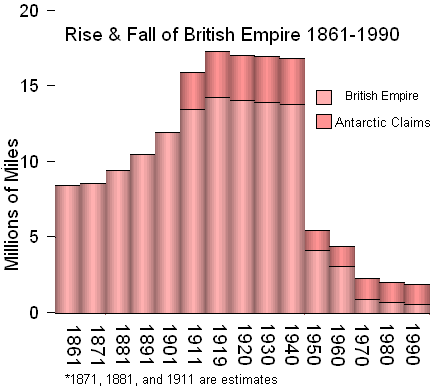
\includegraphics{images/Riseandfall1.png}
\end{center}



In what time interval is the territory of the British Empire growing?  In what time interval is it shrinking?  Let $f(t)$ be the function of land area of the British Empire over time, where $t$ is the current year.  Estimate $f(1940)$ and $f(1950)$.  Find $t$ where $f(t)$ is the highest.

\end{exercise}
\bigskip

\begin{exercise}
Liam weighs 205 pounds and is looking to put on another 10 pounds in muscle over the next 6 months.  He lifts three days per week, and his trends in the past have been to stay at the same weight with a 30-minute workout.  His gain after 6 months is usually one pound for each additional 5 minutes he works out for each session.

How long should he plan to lift each session to meet his goal?
If he plans to lift for 60 minutes each session, how much should he expect to gain in 6 months?
\end{exercise}
\bigskip

\begin{exercise}
Before the beginning of each school year, you, a teacher, need to order enough books for your students, plus a few backup copies.  There are 4 books they each need, and you want 5 replacements for each book, regardless of how many students you have.  Give an equation, table, and graph for this relationship.
\end{exercise}


\pagebreak
\begin{exercise}
To set up your account with the electric company, you must pay a \$90 activation fee.  Your plan is 10 cents per kilowatt-hour.  Additionally, based on information from previous accounts, they have determined that your average bill over the year is \$70.  How much money will you give the electric company this year?  Create a table for the amount you've given the electric company as a function of time.
\end{exercise}



\begin{exercise}
You're considering subscribing to Netflix.  You don't watch very many TV shows, but you watch movies occasionally.  The main competitor for your purposes is Redbox, which rents individual movies for \$1 each.  Netflix is for \$10 each month.

Make a table of the per-month price for each Netflix and Redbox, based on the number of movies you watch each month.  How could this table influence your decision?

\end{exercise}

\begin{exercise}
A local community can estimate their corn yield per acre by keeping track of the greatest number of consecutive days without rain.  They estimate 180 bushels as a high mark, but subtract the greatest number of consecutive days without rain.

How many consecutive days without rain would the community have to have before they estimate only 140 bushels per acre?
\end{exercise}
\bigskip

\begin{exercise}
	The $3^{\prime\prime}$ cactus in my window grows at a rate of $\frac{1}{4}^{\prime\prime}$ per month.  Give an equation, table, and graph which express its height over time.
\end{exercise}
\bigskip

\begin{exercise}

The amount of gas required to start a certain engine is 8 milliliters.  This engine also consumes 0.4 milliliters of gas every second it spends idling.  Create an equation, table, and graph to express this relationship.

\end{exercise}
\bigskip

\begin{exercise}
If a baseball (or, really, any other object) is thrown upward at 40 meters per second, the following equation describes its height as a function of time:

$$f(t) = 2 + 40t - \frac{1}{2}9.8t^2$$

Create a table and a graph for the function.  Make sure to include values of $t$ from 0 to 10.  Using as few math terms as possible, describe what this function is telling us.

\end{exercise}
\bigskip






